% Format verslag in LaTeX maken.
% Lars Aalsma, Tutor Natuur- en Sterrenkunde 2014-2015
% & Ramon Creyghton, tutor Natuur- en Sterrenkunde 2014-2016.
% & David Fokkema, staflid natuurkundepracticum, september 2017.
%
% Dit document mag naar eigen inzicht aangepast en verspreid worden.
% Her en der in dit document staan opmaak-opties en packages opgenomen, die afhankelijk van je voorkeuren kunnen worden aan- of uitgezet. Het is aan te raden je te verdiepen in de werking van deze opties (ze googlen is een start) voor je ze gebruikt.

\documentclass[11pt,a4paper]{article}

\usepackage{fouriernc}        % Dit package kiest het lettertype. Laat dit weg voor standaard Computer Modern.
\usepackage[utf8]{inputenc}   % Je kunt gewóón accenten typen, als je wilt
\usepackage[T1]{fontenc}      % Nodig om de accenten ook ín de pdf te krijgen
\usepackage[dutch]{babel}     % Figuur i.p.v. Figure, en NL afbrekingen
\usepackage{graphicx}         % Voor \includegraphics om figuren in te voegen
\usepackage{amssymb}          % Voor extra symbolen
\usepackage{amsmath}          % Voor extra ondersteuning bij vergelijkingen (zie documentatie)
\usepackage{natbib}           % Voor auteur-jaar citatie.
\usepackage{a4wide}           % Past marges aan voor A4.
\usepackage[small]{caption}   % Voor bijschriften met een iets kleinere lettergrootte dan de hoofdtekst.
\usepackage{url}              % Voor het beter weergeven van url's (lang, of met speciale tekens)
\usepackage{booktabs}         % Voor professionele tabellen
\usepackage[output-decimal-marker={,},list-final-separator={ en }]{siunitx}          % Voor het typesetten en uitlijnen van getallen en eenheden, zie documentatie
\usepackage[pdfusetitle]{hyperref}  % Voor handige links in je PDF. B.v. urls, referenties, etc.
\usepackage[version=4]{mhchem}
\usepackage{physics}


\linespread{1.3}              % Iets grotere regelafstand: fijn voor degene die het nakijkt.

% \renewcommand{\arraystretch}{1.5}   % Om rijen in tabellen wat ruimer rond de tekst te maken.

%% DOCUMENT PROPERTIES % vul in
\title{Analyserapport voor de bepaling van de halfwaardetijd van kalium-40} % Vul in.
\date{\today}

\begin{document}

%% BEGIN TITELPAGINA
\begin{titlepage}
\maketitle
\thispagestyle{empty} % geen paginanummer op de titelpagina

\vfill

% Een samenvatting kun je opnemen op je titelpagina met het commando hieronder. 
%\abstract{\small Lorem ipsum dolor sit amet, consectetur adipiscing elit. Ut tempor ullamcorper sapien, quis lacinia nibh pellentesque vel. Sed ultrices nunc vitae magna pulvinar ac posuere velit bibendum. Nunc placerat ornare libero nec viverra. Nulla ullamcorper diam orci, sit amet scelerisque nisl. Nam sapien felis, auctor vestibulum dignissim nec, egestas eget dolor. \\[2ex]}

 \begin{table}[h]
  \label{tab:credits}
  \begin{tabular}{l l}
   \textsc{Auteur} & Frenk Klein Schiphorst \\
   \textsc{Studentnummer}  & 11866497 \\ % Vul in
   \textsc{Vak} & Natuur- \& Sterrenkunde Practicum 2 \\
   \textsc{Studie} & Natuur- \& Sterrenkunde\\
  \end{tabular}
  \vspace{3ex}
 \end{table}

%De regels hieronder zorgen voor een mooi VU-UvA op je titelpagina. Het bestand logo-combi-vu-uva-nl.png is dan wel noodzakelijk.
%Pro-tip: Bij regelmatig gebruik kan het handig zijn om dit bestand in je 'texmf' folder te zetten (Google is je vriend)
\begin{figure}
  \centering  
  
\includegraphics[width=150mm]{logo-combi-vu-uva-nl}\\   % UvA logo
  \vspace{-13ex}
 \end{figure}

\end{titlepage}
%% EIND TITELPAGINA

\setcounter{page}{2}    % Begin na de titelpagina op pagina 2, dat is iets netter

\suppressfloats[t]      % Nu volgt eigenlijk de eerste pagina van het document. Je wilt dan niet beginnen met een figuur. Dit commando (suppress floats at top of the page) onderdrukt een eventueel figuur en schuift dat naar een andere positie. Dit commando geldt alleen voor de *huidige* pagina.

%%BEGIN VAN DE INHOUD VAN HET DOCUMENT

\section{Inleiding}
In dit analyserapport wordt de bepaling van de halfwaardetijd van kalium-40 gepresenteerd. De gebruikte meetdata bestond uit metingen van de activiteit van bepaalde hoeveelheden kaliumcarbonaat, \ce{K2CO3}. De metingen zijn gedaan met een Geiger-Muller (GM) telbuis.

\section{IJken GM-buis}

Elke GM-buis heeft een efficiëntie, die staat voor de kans dat een deeltje afkomstig van een bron gemeten wordt. De efficiëntie volgt uit
\begin{equation}
\epsilon = \epsilon_g \epsilon_i
\label{eq:efficientie}
\end{equation}
met $\epsilon_g$ de geometrische efficiëntie en $\epsilon_i$ de intrinsieke efficiëntie. De geometrische efficiëntie hangt af van de opstelling, en staat voor de kans dat een deeltje in de richting van het intreevenster uitgezonden wordt. De intrinsieke efficiëntie hangt af van het soort straling.

De intrinsieke efficiëntie van de gebruikte GM-buis is onbekend. Om deze te bepalen zijn ijkmetingen gedaan met zes andere GM buizen. De ijkbron was een strontium-90 bron met bekende activiteit. Aan de hand van een fit is te bepalen of de zevende GM buis, waarmee de metingen aan het kaliumcarbonaat zijn gedaan, ofwel dezelfde intrinsieke efficiëntie had als de andere zes (optie 1), ofwel een iets andere intrinsieke efficiëntie (optie 2). Optie 1 zou betekenen dat de verschillen in de gemeten deeltjes per GM buis alleen veroorzaakt worden door de fout in de telstatistiek. Als dit niet het geval is, geldt optie 2 en wordt voor de intrinsieke efficiëntie van de zevende buis het gemiddelde van de andere zes genomen.

\subsection{Meetdata}
Met elk van de zes GM-buizen is een ijkmeting gedaan. De ijkbron had een activiteit van 1400 Bq. De bron bevond zich op 15,0 cm van het intreevenster van de GM-buis. Het ronde intreevenster had een diameter van 3,0 cm. Ook is er met elke GM-buis een achtergrondmeting gedaan. Alle metingen duurden 480 s. De resultaten van de metingen staan in tabel \ref{tab:tabel1}. De telstatistiek wordt bepaald door de Poissonverdeling. De fout op de getelde deeltjes worden daarom gegeven door de wortel van het aantal getelde deeltjes zelf.

\begin{table}
\caption{Meetdata van de ijkmetingen. De fouten op de aantallen counts worden gegeven door de wortel van het aantal counts zelf.}
\centering
\resizebox{\textwidth}{!}{\begin{tabular}{SSSSS} % uitlijnen als getal, dus met de komma's b.v. recht onder elkaar.
\toprule
{Nummer GM-buis} & {Aantal counts met bron} & {Fout op aantal counts} & {Achtergrondcounts} & {Fout op achtergrond} \\  % Kop moet tussen {} om uitlijning als getal te voorkomen
\midrule
7	&	1399	&	 37.40 	&	187	&	13.67	\\
9	&	1455	&	 38.14 	&	159	&	12.61	\\
10	&	1421	&	 37.70 	&	212	&	14.56	\\
11	&	1580	&	 39.75 	&	154	&	12.41	\\
13	&	1418	&	 37.66 	&	177	&	13.30	\\
15	&	1589	&	 39.86 	&	183	&	13.53	\\
\bottomrule
\end{tabular}}
\label{tab:tabel1}
\end{table}

\subsection{Uitwerking}
Het aantal counts afkomstig van het strontium is te berekenen door het aantal achtergrondcounts van het totale aantal gemeten counts af te halen. De fout hierop wordt bepaald aan de hand van de algemene formule voor foutenpropagatie:
\begin{equation}
\delta q = \sqrt{\left(\pdv{q}{x}\delta x\right)^2 + ... + \left(\pdv{q}{z}\delta z\right)^2}
\label{eq:foutenpropagatie}
\end{equation}

Omschrijven van vergelijking \ref{eq:foutenpropagatie} geeft voor de fout op het aantal counts afkomstig van de strontium-bron:
\begin{equation}
\delta \text{strontium} = \sqrt{\left(\delta \text{counts}\right)^2 + \left(\delta \text{achtergrond}\right)^2}
\label{eq:fout_strontium}
\end{equation}

De totale hoeveelheid deeltjes afkomstig van de strontium-bron is te berekenen. Per vervalsreactie van strontium-90 komen er twee $\beta^-$-deeltjes vrij. Met een activiteit van 1400 Bq en een meetduur van 480 s volgt hieruit voor het totale aantal deeltjes:
\begin{equation}
\text{aantal deeltjes} = 1400 * 2 * 480 = 1.334.000
\label{eq:aantal_deeltjes_ijkbron}
\end{equation}

Op zowel de activiteit van de bron als de duur van de meting zit een fout van 1. Hieruit volgt, via vergelijking \ref{eq:foutenpropagatie}, voor de fout op het totale aantal deeltjes:
\begin{equation}
\text{fout aantal deeltjes} = \sqrt{\left(960\right)^2 + \left(2800\right)^2} = 2960
\end{equation}

Voor de totale efficiëntie van de gebruikte GM-buizen geldt:
\begin{equation}
\epsilon = \frac{\text{aantal gemeten deeltjes}}{\text{totaal uitgezonden deeltjes}}
\label{eq:efficientie_GM}
\end{equation}
Ook hier zit een fout op, die weer volgt uit vergelijking \ref{eq:foutenpropagatie}. Vervolgens is met de geometrische efficiëntie en vergelijking \ref{eq:efficientie} de intrinsieke efficiëntie van de GM-buizen te bepalen. De geometrische efficiëntie is te berekenen als de verhouding tussen de oppervlakte van het intreevenster van de GM-buizen en de oppervlakte van de bolschil waarover de straling vanaf de ijkbron verdeeld wordt. De formule is:
\begin{equation}
\epsilon_g = \frac{\pi r^2}{4\pi R^2}
\label{eq:geometrisch}
\end{equation}
met $r$ de straal van het intreevenster en $R$ de straal van de bolschil. Uiteraard weer met fout volgens vergelijking \ref{eq:foutenpropagatie}. De straal van het intreevenster is hier 1,5 cm, met een fout van 0,1 cm. De straal van de bolschil is gelijk aan de afstand van de bron tot de detector, 15,0 cm, ook met een fout van 0,1 cm. Voor de geometrische efficiëntie van de opstelling geldt dus $\epsilon_g = 0,0025 \pm 0,00033$. De berekende (intrinsieke) efficiënties van de GM-buizen staan in tabel \ref{tab:tabel2}.

\begin{table}
\caption{Berekende efficiënties en intrinsieke efficiënties van de GM-buizen, met de bijbehorende fouten. De intrinsieke efficiëntie is bepaald uit de efficiëntie en de geometrische efficiëntie met vergelijking \ref{eq:efficientie}.}
\centering
\resizebox{\textwidth}{!}{\begin{tabular}{SSSSS} % uitlijnen als getal, dus met de komma's b.v. recht onder elkaar.
\toprule
{Nummer GM-buis} & {$\epsilon$} & {$\delta \epsilon$} & {$\epsilon_i$} & {$\delta \epsilon_i$} \\  % Kop moet tussen {} om uitlijning als getal te voorkomen
\midrule
$7	$&$	0.000902	$&$	0.000030	$&$	0.361	$&$	0.050$	\\
$9	$&$	0.000964	$&$	0.000030	$&$	0.386	$&$	0.053$	\\
$10	$&$	0.000900	$&$	0.000030	$&$	0.360	$&$	0.050$	\\
$11	$&$	0.001061	$&$	0.000031	$&$	0.424	$&$	0.058$	\\
$13	$&$	0.000923	$&$	0.000030	$&$	0.369	$&$	0.051$	\\
$15	$&$	0.001046	$&$	0.000031	$&$	0.418	$&$	0.057$	\\
\bottomrule
\end{tabular}}
\label{tab:tabel2}
\end{table}

Om te bepalen welke van de twee opties (verschillen door telstatistiek of verschillende buizen) geldt, is een constante fit gedaan op het aantal gemeten deeltjes afkomstig van strontium. Als optie 1 (telstatistiek) zou gelden, zou een constante fit een genoeg nauwkeurige representatie van de data geven. De gereduceerde $\chi^2$-waarde van de fit was echter ongeveer 5,5. Op basis hiervan is optie 1 te verwerpen. De intrinsieke efficiëntie van de gebruikte GM-buis wordt dus berekend door het gemiddelde van de zes andere GM-buizen te nemen.

Voor de intrinsieke efficiëntie van de gebruikte GM-buis geldt dus:
\begin{equation}
\epsilon_{i,7} = \frac{1}{6}\sum_{n=1}^{6}\epsilon_{i,n}
\label{eq:intrinsiek_7}
\end{equation}
met $\epsilon_{i,n}$ de intrinsieke efficiëntie van de n-de GM-buis. Voor de fout op de intrinsieke efficiëntie van de 7e buis geldt, via vergelijking \ref{eq:foutenpropagatie}:
\begin{equation}
\delta \epsilon_{i,7} = \frac{1}{6}\sqrt{\sum_{n=1}^{6}\delta\epsilon_{i,n}^2}
\label{eq:intrinsiek_7_err}
\end{equation}

\subsection{Conclusie}
Uit vergelijking \ref{eq:intrinsiek_7} en \ref{eq:intrinsiek_7_err} volgt voor de intrinsieke efficiëntie van de gebruikte GM-buis:
\begin{equation}
\epsilon_i = 0,386 \pm 0,022
\label{eq:intrinsiek_7_waarde}
\end{equation}

\section{Bepaling halfwaardetijd kalium-40}
Voor radioactief verval geldt de volgende relatie voor het aantal kernen op tijdstip t:
\begin{equation}
N(t) = N_0 e^{-\lambda t}
\label{eq:verval}
\end{equation}
met $N_0$ het aantal kernen op tijdstip 0 en $\lambda$ de vervalconstante. Voor $\lambda$ geldt:
\begin{equation}
\lambda = \frac{\ln 2}{\tau_{1/2}}
\label{eq:vervalconstante}
\end{equation}
waarbij $\tau_{1/2}$ de halfwaardetijd van de radioactieve stof is.

De halfwaardetijd van kalium-40 is zeer lang, meer dan een miljard jaar. Het bepalen van de precieze halfwaardetijd gaat dus niet met wachten. Daarvoor is de afgeleide van vergelijking \ref{eq:verval} nodig:
\begin{equation}
\dv{N}{t} = -\lambda N_0 e^{-\lambda t} \approx -\lambda N_0
\label{eq:afgeleide_verval}
\end{equation}
waarbij de uitdrukking achter het $\approx$-teken geldt voor hele lange halfwaardetijden. Het deel voor het $=$-teken in de vergelijking is het totale aantal uitgezonden deeltjes per tijdseenheid. Dit is te berekenen aan de hand van het aantal gemeten deeltjes, de efficiëntie, de duur van de meting en het aantal deeltjes dat per vervalsreactie vrijkomt. De metingen duurden allemaal 600 seconden. Voor kalium-40 is het aantal deeltjes per vervalsreactie 1. Er komt echter maar in 89\% van de gevallen een $\beta^-$-deeltje vrij. Bij de andere 11\% is dit een$\beta^+$-deeltje, wat vrijwel direct zal annihileren met vrije elektronen in de stof/de lucht en dus nooit de detector zal bereiken. Er volgt dus:
\begin{equation}
\dv{N}{t} = \frac{N_\mathrm{gemeten}}{600\cdot\epsilon\cdot 0,89}
\label{eq:afgeleide_verval_2}
\end{equation}

Uit vergelijkingen \ref{eq:vervalconstante}, \ref{eq:afgeleide_verval} en \ref{eq:afgeleide_verval_2} volgt voor de halfwaardetijd:
\begin{equation}
\tau_{1/2} = \frac{N_0 \cdot 600 \cdot \epsilon \cdot 0,89 \cdot \ln 2}{N_\mathrm{gemeten}}
\label{eq:halfwaardetijd}
\end{equation}

\subsection{Meetdata}
De metingen zijn gedaan aan verschillende hoeveelheden kaliumcarbonaat, \ce{K2CO3}. Elke meting duurde 600 s. De resultaten zijn weergegeven in tabel \ref{tab:tabel3}. Ook hier zijn de fouten op de counts gegeven door de wortel van het aantal counts. De fout op het gewicht hangt af van de nauwkeurigheid van de weegschaal, en die bedroeg 0,004 g. Er is ook een achtergrondmeting gedaan, waarbij met een leeg bakje 159 counts gemeten zijn in 600 s. De fout op de achtergrond wordt ook gegeven door de wortel van het aantal counts.

\begin{table}
\caption{Gemeten activiteit van verschillende hoeveelheden \ce{K2CO3}. De fouten op de counts worden gegeven door de wortel van het aantal counts zelf.}
\centering
\resizebox{\textwidth}{!}{\begin{tabular}{SSSS} % uitlijnen als getal, dus met de komma's b.v. recht onder elkaar.
\toprule
{Hoeveelheid \ce{K2CO3} [\si{g}]} & {Fout op \ce{K2CO3} [\si{g}]} & {Aantal counts} & {Fout op counts} \\  % Kop moet tussen {} om uitlijning als getal te voorkomen
\midrule
$	0.171	$&$	0.004	$&$	433	$&$	20.8	$\\
$	0.274	$&$	0.004	$&$	514	$&$	22.7	$\\
$	0.378	$&$	0.004	$&$	651	$&$	25.5	$\\
$	0.632	$&$	0.004	$&$	792	$&$	28.1	$\\
$	1.045	$&$	0.004	$&$	893	$&$	29.9	$\\
$	1.353	$&$	0.004	$&$	939	$&$	30.6	$\\
\bottomrule
\end{tabular}}
\label{tab:tabel3}
\end{table}

\subsection{Aantal kalium-40 deeltjes}
In vergelijking \ref{eq:halfwaardetijd} staat $N_0$ voor het aantal kalium-40 deeltjes in het kaliumcarbonaat. Om dit aantal te berekenen is allereerst de molmassa van kaliumcarbonaat nodig. Uit de molmassa's van kalium, koolstof en zuurstof (en de fouten daarop) volgt:
\begin{equation}
\text{molmassa kaliumcarbonaat} = 138,2058 \pm 0,0011
\label{eq:molmassa_kacarb}
\end{equation}
Door de hoeveelheid \ce{K2CO3} te delen door de molmassa, is het aantal mol kaliumcarbonaat per meting te bepalen. Aangezien er in een mol \ce{K2CO3} twee mol kalium zit, is het aantal mol kalium te bepalen door het aantal mol kaliumcarbonaat te verdubbelen. Uiteraard zijn hier met vergelijking \ref{eq:foutenpropagatie} fouten bij berekend.

Per mol zijn er precies $6,02214076 \cdot 10^{23}$ deeltjes (Getal van Avogadro). Om het aantal kaliumdeeltjes te bepalen moet de hoeveelheid in mol dus vermenigvuldigd worden met het dit getal.

In de natuur is de fractie kalium-40 ten opzichte van de totale hoeveelheid kalium ongeveer $1,17 \cdot 10^{-4}$, met een fout van 
$0,01 \cdot 10^{-4}$. Om het totale aantal kalium-40 deeltjes per meting te berekenen, moet het totale aantal kaliumdeeltjes vermenigvuldigd worden met deze fractie. De resultaten hiervan staan in tabel \ref{tab:tabel4}. De fout is weer berekend met vergelijking \ref{eq:foutenpropagatie}.

\begin{table}
\caption{Aantal kalium-40 deeltjes per hoeveelheid \ce{K2CO3}.}
\centering
\resizebox{\textwidth}{!}{\begin{tabular}{SSS} % uitlijnen als getal, dus met de komma's b.v. recht onder elkaar.
\toprule
{Hoeveelheid \ce{K2CO3} [\si{g}]} & {Aantal kalium-40 deeltjes} & {Fout op aantal kalium-40}\\  % Kop moet tussen {} om uitlijning als getal te voorkomen
\midrule
$	0.171	$&$	1.744E+17	$&$	4.342E+15	$\\
$	0.274	$&$	2.794E+17	$&$	4.726E+15	$\\
$	0.378	$&$	3.854E+17	$&$	5.243E+15	$\\
$	0.632	$&$	6.444E+17	$&$	6.853E+15	$\\
$	1.045	$&$	1.066E+18	$&$	9.978E+15	$\\
$	1.353	$&$	1.380E+18	$&$	1.248E+16	$\\
\bottomrule
\end{tabular}}
\label{tab:tabel4}
\end{table}

\subsection{Bepaling halfwaardetijd per meting}
In vergelijking \ref{eq:halfwaardetijd} staat ook het aantal gemeten deeltjes. Dit is per meting te berekenen door het aantal achtergrondcounts van het totale aantal gemeten counts af te halen. 

De efficiëntie volgt uit vergelijking \ref{eq:efficientie}. De intrinsieke efficiëntie is bepaald bij vergelijking \ref{eq:intrinsiek_7_waarde}. De geometrische efficiëntie moet echter geschat worden. Uit de opstelling volgt een geometrische efficiëntie rond 0,4, met een fout van 0,07. Deze waardes zijn gekozen omdat er in ieder geval minder dan de helft van de straling het intreevenster binnen komt. Het lijkt echter ook in ieder geval meer dan een derde te zijn, omdat de bron wel vrij dicht op het venster staat. Daarom is deze geometrische efficiëntie gekozen, met een relatief grote fout omdat het een ruwe schatting betreft.

Met het aantal kalium-40 deeltjes, het aantal gemeten deeltjes en de efficiëntie is nu de halfwaardetijd per meting te berekenen. Voor de fout op de halfwaardetijd kan weer vergelijking \ref{eq:foutenpropagatie} gebruikt worden. Door de vele variabelen is echter gekozen voor de versimpelde vorm:
\begin{equation}
\frac{\delta \tau_{1/2}}{\tau_{1/2}} = \sqrt{(\frac{\delta N_0}{N_0})^2 + (\frac{\delta \epsilon}{\epsilon})^2 + (\frac{\delta t}{t})^2 (\frac{\delta N_\mathrm{gemeten}}{N_\mathrm{gemeten}})^2}
\label{eq:foutenpropagatie_2}
\end{equation}
met $t$ de duur van het experiment in seconden. Vervolgens is de halfwaardetijd omgerekend naar jaren door te delen door een factor $(365,25 \cdot 24 \cdot 60 \cdot 60)$. De resultaten per meting staan in tabel \ref{tab:tabel5}.

\begin{table}
\caption{Berekende halfwaardetijden bij verschillende metingen.}
\centering
\resizebox{\textwidth}{!}{\begin{tabular}{SSS} % uitlijnen als getal, dus met de komma's b.v. recht onder elkaar.
\toprule
{Hoeveelheid \ce{K2CO3} [\si{g}]} & {Halfwaardetijd [jaar]} & {Fout halfwaardetijd [jaar]}\\  % Kop moet tussen {} om uitlijning als getal te voorkomen
\midrule
$	0.171	$&$	1.154E+09	$&$	2.371E+08	$\\
$	0.274	$&$	1.427E+09	$&$	2.830E+08	$\\
$	0.378	$&$	1.420E+09	$&$	2.741E+08	$\\
$	0.632	$&$	1.846E+09	$&$	3.512E+08	$\\
$	1.045	$&$	2.632E+09	$&$	4.977E+08	$\\
$	1.353	$&$	3.206E+09	$&$	6.051E+08	$\\
\bottomrule
\end{tabular}}
\label{tab:tabel5}
\end{table}

\subsection{Berekening halfwaardetijd}
Wat opvalt is dat de halfwaardetijd stijgt bij grotere hoeveelheden kaliumcarbonaat. Dit is het gevolg van zelfabsorptie, waarbij uitgezonden elektronen geabsorbeerd worden in de stof voordat ze de detector bereiken. Hoe dikker de laag kaliumcarbonaat, hoe meer zelfabsorptie plaatsvindt. Het aantal gemeten deeltjes is dan kleiner en uit vergelijking \ref{eq:halfwaardetijd} volgt dan een grotere halfwaardetijd. Dit is een exponentieel verband. Om de werkelijke halfwaardetijd te berekenen kan er dus een exponentiële fit gedaan worden over de verkregen data. De gebruikte formule om te fitten is:
\begin{equation}
\tau_{1/2, \mathrm{gemeten}} = \tau_{1/2, \mathrm{werkelijk}} \cdot e^{\mu x}
\label{eq:fit_halfwaarde}
\end{equation}
waarbij de werkelijke waarde voor $\mu$ niet uitmaakt. De fit hoeft dus ook niet goed te zijn, het gaat alleen om de beginwaarde, $\tau_{1/2, \mathrm{werkelijk}$.

In figuur \ref{fig:figuur1} is de gebruikte fit te zien. Uit de fit is gekomen:
\begin{equation*}
\tau_{1/2} = 1,058 \cdot 10^9 \text{ jaar} \pm 4,036 \cdot 10^7 \text{ jaar}
\end{equation*}

\begin{figure}  % Forceer je figuur niet naar [h]ere. Dat gebeurt in artikelen ook niet.
\centering
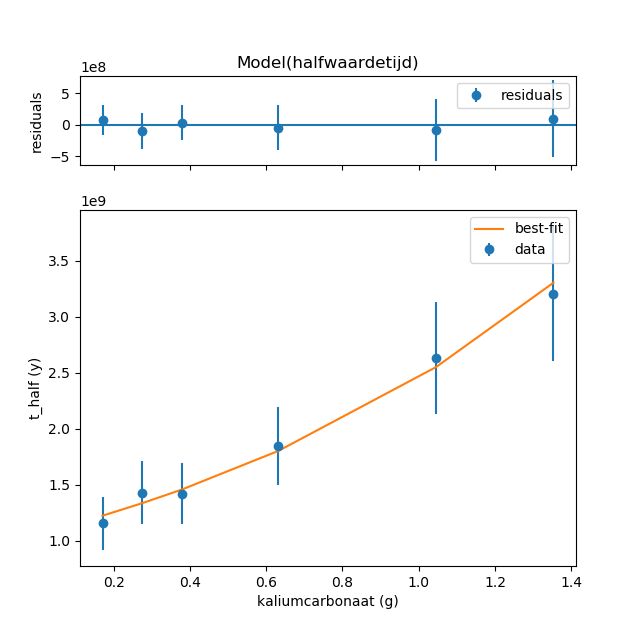
\includegraphics[scale=0.7]{fit_halfwaarde}
\caption{Fit om de halfwaardetijd te berekenen.}
\label{fig:figuur1}
\end{figure}

\section{Conclusie & Discussie}
De theoretische waarde voor de halfwaardetijd van kalium-40 is ongeveer $1,25 \cdot 10^9$ jaar. De gevonden waarde ligt dus wel in dezelfde orde van grootte.

Het verschil tussen de gevonden en de theoretische waarde komt waarschijnlijk voornamelijk door de schatting van de intrinsieke efficiëntie van de gebruikte GM-buis. Tijdens de data-analyse bleek een verschil van 0,02 in de gebruikte intrinsieke efficiëntie al een aanzienlijk verschil te maken voor de uitkomst. Met een intrinsieke efficiëntie van 0,41, tegenover de gebruikte 0,386, werd een waarde voor de halfwaardetijd gevonden rond $1,23 \cdot 10^9$, veel dichter bij de theoretische waarde. In een vervolgonderzoek zou de waarde van de gebruikte GM-buis daarom bepaald moeten worden door direct een meting te doen aan de ijkbron, zodat de intrinsieke efficiëntie van de GM-buis berekend kan worden in plaats van geschat.


%\section{Inleiding}
%
%Lorem ipsum dolor sit amet, consectetur adipiscing elit. Ut tempor ullamcorper sapien, quis lacinia nibh pellentesque vel. Sed ultrices nunc vitae magna pulvinar ac posuere velit bibendum. Nunc placerat ornare libero nec viverra. Nulla ullamcorper diam orci, sit amet scelerisque nisl. Nam sapien felis, auctor vestibulum dignissim nec, egestas eget dolor. Suspendisse iaculis, diam pulvinar luctus iaculis, ipsum nisl consectetur nisi, a lacinia eros lacus vitae dui. In fermentum ante quis ante porttitor congue. Mauris sollicitudin rhoncus dictum. Donec pretium molestie tempus. Integer suscipit egestas erat sit amet volutpat. Nullam et magna risus. Nam vel nisi libero. Duis ultricies ipsum eu lorem congue vestibulum. Aenean ut felis velit, ac lacinia erat. In a dolor dignissim elit faucibus facilisis. Vivamus iaculis ornare lacus, viverra convallis sapien pulvinar vitae.
%
%\section{Figuren en tabellen}
%Een voorbeeld van een figuur is op de volgende pagina gegeven, zie figuur \ref{fig:figuur1}. Figuren staan nóóit in de lopende tekst. Pak een willekeurig artikel en je zult zien dat figuren óf bovenaan een pagina staan, óf onderaan een pagina, óf op een eigen pagina. Nooit in het midden. Probeer dus ook niet met \verb|[h]| o.i.d. de plaatsing van figuren te forceren. Over het algemeen maak je het alleen maar erger.
%
%\begin{figure}  % Forceer je figuur niet naar [h]ere. Dat gebeurt in artikelen ook niet.
%\centering
%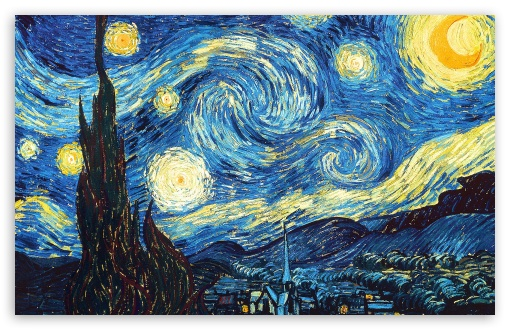
\includegraphics[scale=0.5]{figuur1}
%\caption{Een figuur heeft een onderschrift. Een plaatje trekt al snel je aandacht weg van de hoofdtekst. Zodra je het plaatje snel bekeken hebt, is de natuurlijke neiging om `verder te lezen' en beweegt je aandacht naar onder het plaatje. Als dáár dan een stukje tekst met uitleg staat, wordt het sneller gelezen dan wanneer dat bóven de figuur staat. Blijkt uit onderzoek.}
%\label{fig:figuur1}
%\end{figure}
%
%Een voorbeeld van een tabel is hieronder gegeven, zie tabel \ref{tab:tabel1}.
%
%\begin{table}
%\caption{Een tabel heeft een bovenschrift. Een plaatje of tabel (met veel witruimte eromheen) trekt al snel je aandacht weg van de hoofdtekst. Toch worden je ogen al snel richting de kop getrokken (wat staat er boven de kolommen?) en als dáár dan een stukje tekst met uitleg staat, lees je dat sneller dan wanneer het ónder de tabel staat. Blijkt uit onderzoek.}
%\centering
%\begin{tabular}{SS} % uitlijnen als getal, dus met de komma's b.v. recht onder elkaar.
%\toprule
%{Slingerlengte [\si{\centi\meter}]} & {Slingertijd [\si{\second}]} \\  % Kop moet tussen {} om uitlijning als getal te voorkomen
%\midrule
%5 & 4.5 \\
%10 & 6.3 \\
%15 & 7.8 \\
%20 & 9.0 \\
%25 & 10.0 \\
%\bottomrule
%\end{tabular}
%\label{tab:tabel1}
%\end{table}
%
%\section{Een sectie}
%
%Formules in \LaTeX\ gaan vanzelf al snel goed. Zo krijgt iedere vergelijking automatisch een nummer, dat keurig rechts wordt uitgelijnd. Menig student krijgt dat in Word o.i.d. niet goed voor elkaar. Denk er wel aan formules op te nemen in de lopende tekst.
%\begin{equation}
%  F = ma
%  \label{eq:eerste-wet-newton}
%\end{equation}
%De eerste wet van Newton. Vergelijking \ref{eq:eerste-wet-newton} is níet opgenomen in de lopende tekst, en dat leest dus niet zo lekker door. Je moet jezelf afvragen: kan ik dit verhaal voorlezen? Als je het verhaal goed kunt voorlezen \emph{inclusief} de vergelijking, zonder haperingen, dan staat het goed.
%
%Zo is bijvoorbeeld de trillingstijd van een slinger gegeven door
%\begin{equation}
%  T = 2\pi\sqrt{\frac{l}{g}},
%  \label{eq:trillingstijd-slinger}
%\end{equation}
%met de trillingstijd $T$, de lengte van de slinger $l$ en de valversnelling $g$. Let ook op de komma aan het eind van vergelijking~\ref{eq:trillingstijd-slinger}. Dit stukje tekst kun je vloeiend voorlezen, zonder haperingen. Geef je vergelijkingen ook \emph{namen} om aan te refereren, en geen \emph{nummers}.
%
%Lorem ipsum dolor sit amet, consectetur adipiscing elit. Ut tempor ullamcorper sapien, quis lacinia nibh pellentesque vel. Sed ultrices nunc vitae magna pulvinar ac posuere velit bibendum. Nunc placerat ornare libero nec viverra. Nulla ullamcorper diam orci, sit amet scelerisque nisl. Nam sapien felis, auctor vestibulum dignissim nec, egestas eget dolor. Suspendisse iaculis, diam pulvinar luctus iaculis, ipsum nisl consectetur nisi, a lacinia eros lacus vitae dui. In fermentum ante quis ante porttitor congue. Mauris sollicitudin rhoncus dictum. Donec pretium molestie tempus. Integer suscipit egestas erat sit amet volutpat. Nullam et magna risus. Nam vel nisi libero. Duis ultricies ipsum eu lorem congue vestibulum. Aenean ut felis velit, ac lacinia erat. In a dolor dignissim elit faucibus facilisis. Vivamus iaculis ornare lacus, viverra convallis sapien pulvinar vitae.
%
%\section{Referentie voorbeelden}
%
%\citet{Kachru2003} hebben aangetoond dat de Sitter vacua voorkomen in snaartheorie. Dit werd echter in een latere publicatie tegengesproken \citep{Bena2010}.
%
%%Refereren met LaTeX kan op twee manieren, zie ook Hoofdstuk 5 van de handleiding AVT. Hier voegen we referenties handmatig toe door gebruik te maken van thebibliography, zie de regels hieronder beginnend bij \begin{thebibliography}{}. Elke nieuwe referentie wordt toegevoegd met \bibitem.
%
%%In een \bibitem geeft de tekst tussen de [...] aan hoe de referentie verschijnt in de tekst. Tussen de {...} staat het label waarmee in de tekst naar de referentie kan worden verwezen. Refereren in de tekst wordt gedaan zoals hierboven (met \citet{<label>} en \citep{<label>}).



\end{document}
